\documentclass{beamer}
%%%%%%%%%%%%%%%%%%%%%%%%%%%%%%%%%%%%%%%%%%%%%%%%%%%%%%%%%%%%%%%%%%%%%%%%%%%%%%
% Colours, text macros and similar stuff
%%%%%%%%%%%%%%%%%%%%%%%%%%%%%%%%%%%%%%%%%%%%%%%%%%%%%%%%%%%%%%%%%%%%%%%%%%%%%%

\usepackage{tikz}
\usetikzlibrary{calc}

%%%%%%%%%%%%%%%%%%%%%%%%%%%%%%%%%%%%%%%%%%%%%%%%%%%%%%%%%%%%%%%%%%%%%%%%%%%%%%
% Colours, text macros and similar stuff
%%%%%%%%%%%%%%%%%%%%%%%%%%%%%%%%%%%%%%%%%%%%%%%%%%%%%%%%%%%%%%%%%%%%%%%%%%%%%%

\definecolor{AltranTitle}{RGB}{139,129,120}
\definecolor{AltranSubtitle}{RGB}{115,124,130}
\definecolor{AltranGrey}{RGB}{89,89,89}

\definecolor{AnColour01}{RGB}{92,127,146} % Institutional grey
\definecolor{AnColour02}{RGB}{48,149,180} % Institutional blue

\definecolor{AnGrey01}{RGB}{213,210,202} % Warm Grey 2   - lightest
\definecolor{AnGrey02}{RGB}{199,194,186} % Warm Grey 3
\definecolor{AnGrey03}{RGB}{183,177,169} % Warm Grey 4
\definecolor{AnGrey04}{RGB}{165,157,149} % Warm Grey 6
\definecolor{AnGrey05}{RGB}{139,129,120} % Warm Grey 8   - darkest

\definecolor{AnSecondary01}{RGB}{203,0,68}   % Pinkish
\definecolor{AnSecondary02}{RGB}{190,214,0}  % Greenish
\definecolor{AnSecondary03}{RGB}{142,37,141} % Purplish
\definecolor{AnSecondary04}{RGB}{240,171,0}  % Yellowish

% Same as above with some names
\definecolor{AnSecondaryRed}{RGB}{203,0,68}      % Pinkish
\definecolor{AnSecondaryGreen}{RGB}{190,214,0}   % Greenish
\definecolor{AnSecondaryPurple}{RGB}{142,37,141} % Purplish
\definecolor{AnSecondaryYellow}{RGB}{240,171,0}  % Yellowish

% A very light grey for pxcode
\definecolor{CodeBG}{rgb}{0.95,0.95,0.95}

% Backwards compatibility
\definecolor{PraxisPurple}{RGB}{48,149,180}  % AnColour02
\definecolor{PraxisPink}{RGB}{92,127,146}    % AnColour01

\newcommand{\company}[0]{Altran}
\newcommand{\companyFormal}[0]{Altran UK Limited}
\newcommand{\companyAddress}[0]{22 St Lawrence Street, SouthGate, Bath, BA1 1AN}


\newcommand{\spark}[0]{{\sc Spark}}

\newcommand{\gps}[0]{GPS}

\newcommand{\checker}[0]{Checker}
\newcommand{\examiner}[0]{Examiner}
\newcommand{\isabelle}[0]{Isabelle/HOL}
\newcommand{\pogs}[0]{POGS}
\newcommand{\riposte}[0]{Riposte}
\newcommand{\simplifier}[0]{Simplifier}
\newcommand{\sparkclean}[0]{SPARKClean}
\newcommand{\sparkformat}[0]{SPARKFormat}
\newcommand{\sparkmake}[0]{SPARKMake}
\newcommand{\sparksimp}[0]{SPARKSimp}
\newcommand{\victor}[0]{Victor}
\newcommand{\zombiescope}[0]{ZombieScope}

\usepackage{listings}

\font\btt=cmbtt8
\lstdefinestyle{pxstyle}
   {basicstyle=\scriptsize\ttfamily,
    keywordstyle=\btt\color{AnColour02},
    commentstyle=\rmfamily\it\color{AltranGrey},
    captionpos=b,
    caption={},label={},
    numbers=none,
    escapeinside={(*}{*)}}

\lstset{defaultdialect=[LaTeX]TeX}

\lstdefinelanguage{fdl}{
  morekeywords={function,type,array,record,const,pending,var,and,or,not,for_some,for_all,
                element,update,
                may_be_replaced_by,may_be_deduced,may_be_deduced_from,are_interchangeable,if,
                goal,checktype},
  morecomment=[s]{/*}{*/}
}

%% Needs dialects for SPARK83, SPARK95 and SPARK2005
%% and some work on getting the annotation keywords to be highlighted (pun intended)
\lstdefinelanguage{SPARK}{
  language = [95]Ada,
  morekeywords = {pre,post,assert,assume,check,derives,hide,global,depends,inherit,from,own,initializes,main_program,assert,loop_variant,loop_invariant,increases,decreases,ghost,abstract_state,refined_state,refined_global,refined_depends},
  comment=[l][commentstyle]{--\ },
  texcl=true,
  showstringspaces=false
}

\lstdefinelanguage{SMTLIB}{
  language = LISP,
  morekeywords = {set-logic,
                  declare-const,declare-fun,define-const,define-fun,
                  check-sat,
                  get-value,
                  exit},
  texcl=true,
  showstringspaces=false
}


\lstdefinelanguage{indexfile}{
  morekeywords = {spec,is,in,body,specification,superindex,auxindex,components,are},
  comment=[l][commentstyle]{--\ },
  texcl=true,
  showstringspaces=false
}

\lstdefinelanguage{cmdline}{
  comment=[l][commentstyle]{--\ },
  texcl=true,
  showstringspaces=false
}

\lstnewenvironment{pxcode}[1][\@empty]{
  \lstset{language=}
  \lstset{style=pxstyle}
  \ifx#1\@empty\else
  \lstset{#1}
  \fi
}{%
}

\lstset{style=pxstyle}

\lstdefinelanguage{BNF}{
  language = [2005]Ada,
  deletecomment = [l]{--},
  morekeywords = {check,assert,pre,post},
  moredelim=[is][\emph]{//}{//},
}

% A smaller style than default, this is useful if you have a lot of
% code to typeset on a slide
\lstdefinestyle{tinystyle}
   {basicstyle=\tiny\tt,
    keywordstyle=\color{AnColour02},
    commentstyle=\rmfamily\it\color{AltranGrey},
    captionpos=b,
    caption={},label={},
    numbers=none,
    escapeinside={(*}{*)}}


\newenvironment{changemargin}[2]{%
  \begin{list}{}{%
    \setlength{\topsep}{0pt}%
    \setlength{\leftmargin}{#1}%
    \setlength{\rightmargin}{#2}%
    \setlength{\listparindent}{\parindent}%
    \setlength{\itemindent}{\parindent}%
    \setlength{\parsep}{\parskip}%
  }%
  \item[]}{\end{list}}

%%%%%%%%%%%%%%%%%%%%%%%%%%%%%%%%%%%%%%%%%%%%%%%%%%%%%%%%%%%%%%%%%%%%%%%%%%%%%%
% Altran style
%%%%%%%%%%%%%%%%%%%%%%%%%%%%%%%%%%%%%%%%%%%%%%%%%%%%%%%%%%%%%%%%%%%%%%%%%%%%%%

% We are going to position text at absolute positions on each frame.
\usepackage{textpos}

% Provide an optional \subtitle command
\gdef\thesubtitle{\ }
\def\subtitle#1{\gdef\thesubtitle{#1\\}}

% Use square shapes (in particular for bullet points)
\useinnertheme{rectangles}
\usecolortheme[named=AnColour02]{structure}    % Lighter

\setbeamercolor{block title}{use=structure,fg=white,bg=structure}
\setbeamercolor{block body}{parent=normal text,use=block title,bg=AnGrey01!40}


% The frametitle is not put in the top-left corner, but is a bit
% offset.
\setbeamertemplate{frametitle}
{
  \begin{textblock*}{\textwidth}(-0.5cm,0.5cm)
    {\rm\insertframetitle}\\
    \vskip -2mm
    {\color{AltranSubtitle}\small\insertframesubtitle}
  \end{textblock*}
  \vskip1cm
}

% No navigation symbols
\setbeamertemplate{navigation symbols}{}

% Use Altran colours throughout
\setbeamercolor*{palette quaternary}{bg=AnColour01,fg=white} % Top part

% Standard background picture
\usebackgroundtemplate{%
\begin{tikzpicture}
\node[minimum width=\paperwidth,minimum height=\paperheight-0.1pt] (page) {};
\coordinate (origin) at ($(page.south west) + (0pt, 0pt)$);
\coordinate (a) at ($(origin) + 0.9*(0cm, 1cm)$);
\coordinate (b) at ($(origin) + 0.9*(1.07cm, 0.26cm)$);
\coordinate (c) at ($(origin) + 0.9*(2.5cm, 0cm)$);
\draw[fill,AnColour02] (a) -- (b) -- (origin) -- cycle;
\draw[fill,AnGrey01] (origin) -- (b) -- (c) -- cycle;
\node[anchor=south east] at (page.south east) {
\includegraphics[width=2cm]{altran_rgb.pdf}};
\end{tikzpicture}%
}

% Page number in white
\defbeamertemplate*{footline}{AltranFooter}
{
  \hskip0.2cm{\color{white}\insertframenumber}%
  \vskip0.35cm
}
\usebeamertemplate{AltranFooter}

\setbeamertemplate{note page}
{
  \vskip0.5cm
  \begin{changemargin}{-0.5cm}{-0.5cm}
    \scriptsize\setlength\parskip{3pt}
    \insertnote
  \end{changemargin}
}


% Title page stuff.
\renewcommand{\titlepage}
{
  \begin{textblock*}{\textwidth}(0cm,-2cm)
    \flushright
    {
      \LARGE
      \color{AltranTitle}
      \rm
      \inserttitle\\
    }
    \vspace{0.1cm}
    \begin{minipage}{7.5cm}
      \flushright
      \color{AltranSubtitle}
      \thesubtitle
    \end{minipage}\\
    \vspace{0.1cm}
    {
      \scriptsize
      \insertdate
    }
  \end{textblock*}
}

\def\titleprismlabela#1{\gdef\tprismla{#1}}
\def\titleprismlabelb#1{\gdef\tprismlb{#1}}
\def\titleprismlabelc#1{\gdef\tprismlc{#1}}

\newenvironment{altrantitle}
{
  \gdef\tprismla{SPARK}
  \gdef\tprismlb{Correctness by Construction}
  \gdef\tprismlc{Formal Methods}
}
{
  {
    \usebackgroundtemplate{
\includegraphics[width=\paperwidth]{pres_title.png}}
    \begin{frame}
      \titlepage
      \begin{textblock*}{4cm}(-3.3cm,-1.5cm)
        \tiny\flushright\tprismla
      \end{textblock*}
      \begin{textblock*}{4cm}(0.6cm,3.6cm)
        \tiny\tprismlb
      \end{textblock*}
      \begin{textblock*}{4cm}(4cm,2.7cm)
        \tiny\tprismlc
      \end{textblock*}
    \end{frame}
  }
}

\renewcommand{\maketitle}{
  \begin{altrantitle}
  \end{altrantitle}
}

% The backpage is automatically added as the last slide
\newcommand{\finalslide}
{
  \usebackgroundtemplate{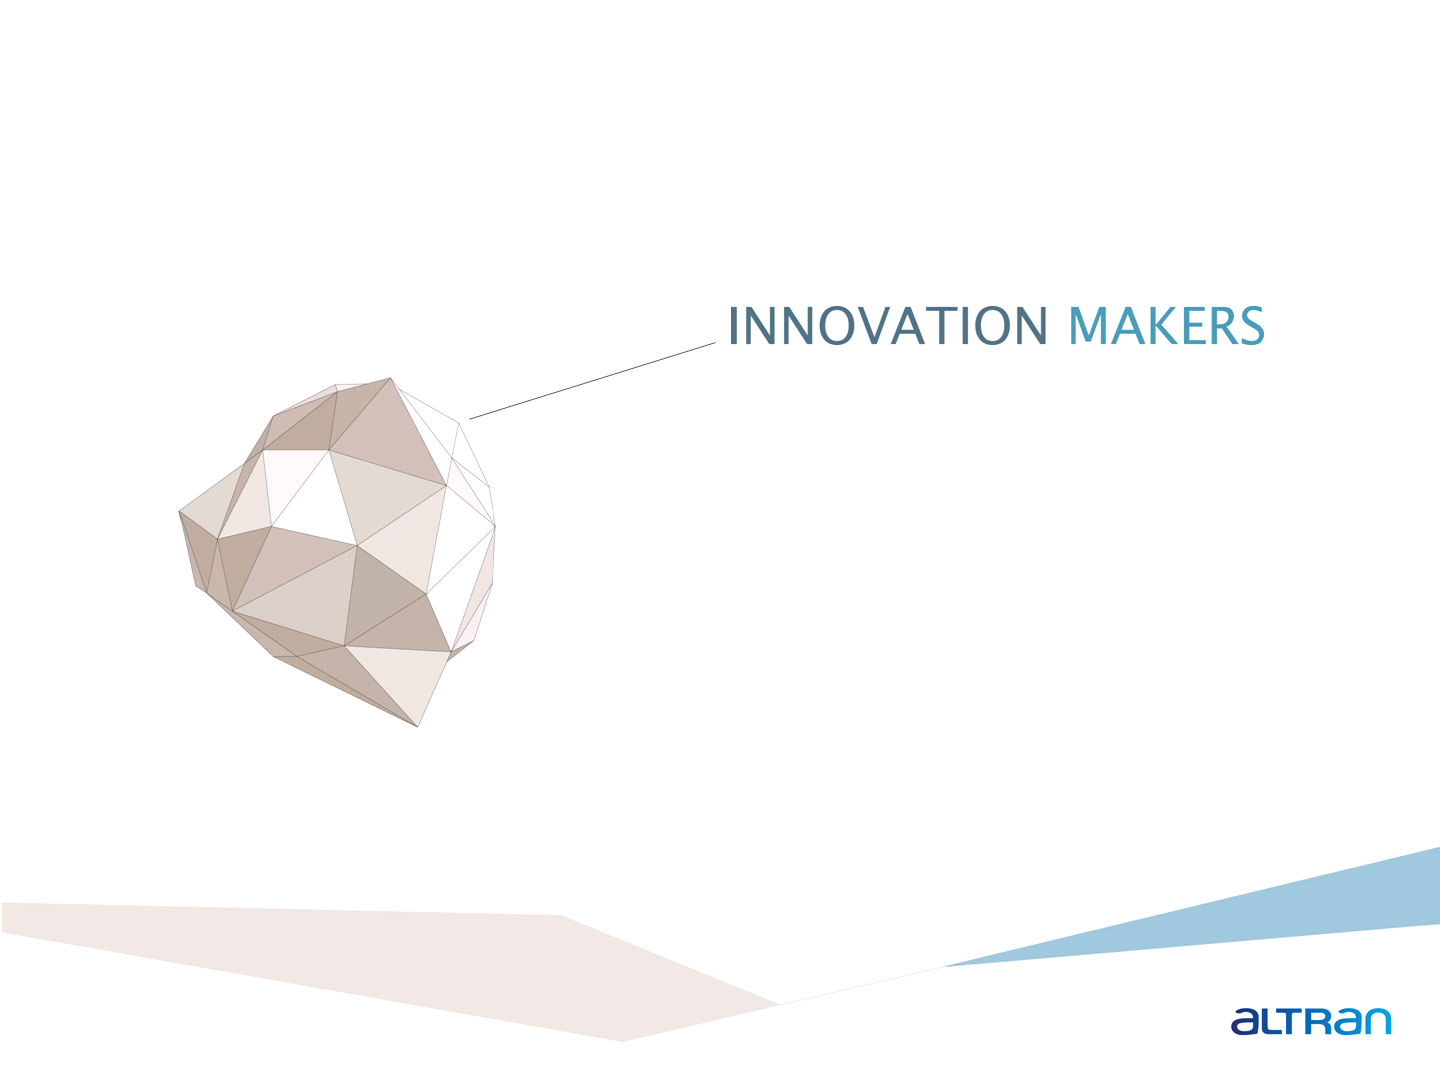
\includegraphics[width=\paperwidth]{pres_back.png}}
  \begin{frame}
  \end{frame}
}
\AtEndDocument{\finalslide}

\usepackage{listings}
\usepackage{setspace}
\usepackage{tikz}
\usepackage{lcd}
\usepackage{pgflibraryshapes}
\usepackage{rotating}
\usetikzlibrary{calc,fit,shapes,arrows}
\usetikzlibrary{backgrounds,shadows}

\setbeamertemplate{note page}[plain]
\setbeameroption{show notes}


\lstdefinestyle{tinystyle} {basicstyle=\scriptsize\tt,
  keywordstyle=\bf, commentstyle=\rmfamily\it, escapeinside={(*}{*)}}
\lstset{style=tinystyle}

\lstdefinelanguage{SPARK}{ language = [95]Ada, morekeywords = {pre,
    post, assert, assume, check, derives, hide, global, inherit, from,
    own, initializes, main_program, input, output, in_out,
    refined_pre, refined_post, some, depends}, comment=[l][commentstyle]{--\ },
  showstringspaces=false }

\lstset{language=SPARK}

\title{Optimising Verification Effort\\with SPARK 2014}
\subtitle{Andrew Hawthorn}
\hypersetup{colorlinks=true}
\date{12th November 2013}
\begin{document}

\begin{altrantitle}
  \titleprismlabela{Formally Specify}
  \titleprismlabelb{Test and Prove}
  \titleprismlabelc{Reduce Cost}
\end{altrantitle}

%\begin{frame}[fragile]{Contents}
%  \tableofcontents
%\end{frame}

\makeatletter
\newenvironment{btHighlight}[1][]
{\begingroup\tikzset{bt@Highlight@par/.style={#1}}\begin{lrbox}{\@tempboxa}}
{\end{lrbox}\bt@HL@box[bt@Highlight@par]{\@tempboxa}\endgroup}

\newcommand\btHL[1][]{%
  \begin{btHighlight}[#1]\bgroup\aftergroup\bt@HL@endenv%
}
\def\bt@HL@endenv{%
  \end{btHighlight}%
  \egroup
}
\newcommand{\bt@HL@box}[2][]{%
  \tikz[remember picture]{%
    \pgfpathrectangle{\pgfpoint{1pt}{0pt}}{\pgfpoint{\wd #2}{\ht #2}}%
    \pgfusepath{use as bounding box}%
    \node[anchor=base west,%
          outer sep=0pt,%
          inner xsep=1pt,%
          inner ysep=0pt,%
          rounded corners=2pt,%
          minimum height=\ht\strutbox+1pt,%
          #1]%
          {%
            \raisebox{1pt}{\strut}\strut\usebox{#2}%
          };%
  }%
}
\makeatother

\section{Introduction}

\begin{frame}[fragile]{Summary of talk}
  \begin{itemize}
  \item Formality of analysis can be tailored to project needs
  \item Combining Test and proof reduces verification effort
  \item Using contracts makes it easier to parallelise verification
  \end{itemize}
\end{frame}

\begin{frame}[fragile]{Agenda}
  \begin{itemize}
     \item Setting the foundations for proof and test
     \item Incremental analysis - the verification spectrum
     \item How proof supports test
     \item Proof and test scenarios
     \item Only test
     \item Test to prove contracts
     \item Test to debug contracts
     \item Only prove
     \item Prove and test
     \item Conclusions
  \end{itemize}
\note[item]{Don't talk through this slide, move onto the next slide straight away}
\end{frame}

\begin{frame}[fragile]{SPARK 2014 language evolution}
\note[item]<1>{Duality of execution and proof of contracts changes the game}
  \begin{changemargin}{-0.75cm}{-0.75cm}
    \begin{center}
      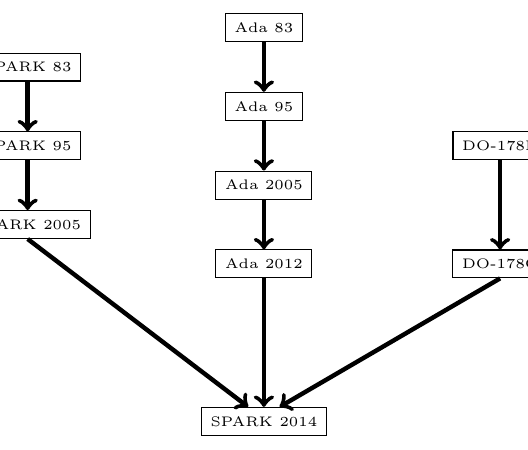
\begin{tikzpicture}[font=\tiny,y=0.95cm]
        \useasboundingbox (-3cm,-5cm) rectangle (3cm,0cm);

        % SPARK stream
        \node<2->[rectangle, draw] (s83) at (-3cm,-0.5cm) {SPARK 83};
        \node<3->[rectangle, draw] (s95) at (-3cm,-1.5cm) {SPARK 95};
        \node<4->[rectangle, draw] (s05) at (-3cm,-2.5cm) {SPARK 2005};
        \node<8->[rectangle, draw] (s12) at (-0cm,-5cm) {SPARK 2014};

        % SPARK stream
        \node<1->[rectangle, draw] (ada83) at (-0cm,-0cm) {Ada 83};
        \node<3->[rectangle, draw] (ada95) at (-0cm,-1cm) {Ada 95};
        \node<4->[rectangle, draw] (ada05) at (-0cm,-2cm) {Ada 2005};
        \node<5->[rectangle, draw] (ada12) at (-0cm,-3cm) {Ada 2012};

        % Standards stream
        \node<6->[rectangle, draw] (178b) at ( 3cm,-1.5cm) {DO-178B};
        \node<7->[rectangle, draw] (178c) at ( 3cm,-3cm) {DO-178C};

        % arrows
        \draw<3->[ultra thick][->] (s83.south) to (s95.north);
        \draw<4->[ultra thick][->] (s95.south) to (s05.north);
        \draw<8->[ultra thick][->] (s05.south) to ([xshift=-0.2cm]s12.north);

        \draw<3->[ultra thick][->] (ada83.south) to (ada95.north);
        \draw<4->[ultra thick][->] (ada95.south) to (ada05.north);
        \draw<5->[ultra thick][->] (ada05.south) to (ada12.north);
        \draw<8->[ultra thick][->] (ada12.south) to (s12.north);

        \draw<7->[ultra thick][->] (178b.south) to (178c.north);
        \draw<8->[ultra thick][->] (178c.south) to ([xshift=0.2cm]s12.north);

      \end{tikzpicture}
    \end{center}
  \end{changemargin}
\end{frame}

\begin{frame}{Setting the foundations for proof and test}
  \note[item]<1>{Key messages: If you are thinking about combining proof and test, ake sure you consider it at the start of your project}
  \note[item]<1>{NB this is not the only lifecycle}
  \note[item]<1>{SPARK often seen as just a coding language}
  \note[item]<1>{Ada 2012 supports contract execution}
  \note[item]<1>{Proof means SPARK also covers unit verification}
  \note[item]<1>{Proof implies formal specification which brings SPARK into LLRs}
  \note[item]<1>{NB review of Tokeneer Z suggests writing spec in SPARK isn't any more challenging than writing in Z but provides plenty of benefits (eg don't need to respecify to prove properties, rapid prototyping options available etc)}
  \note[item]<1>{Modular verification means SPARK can be applied at architecture and architecture can be verified statically}
  \begin{changemargin}{-0.75cm}{-0.75cm}
    \begin{center}
      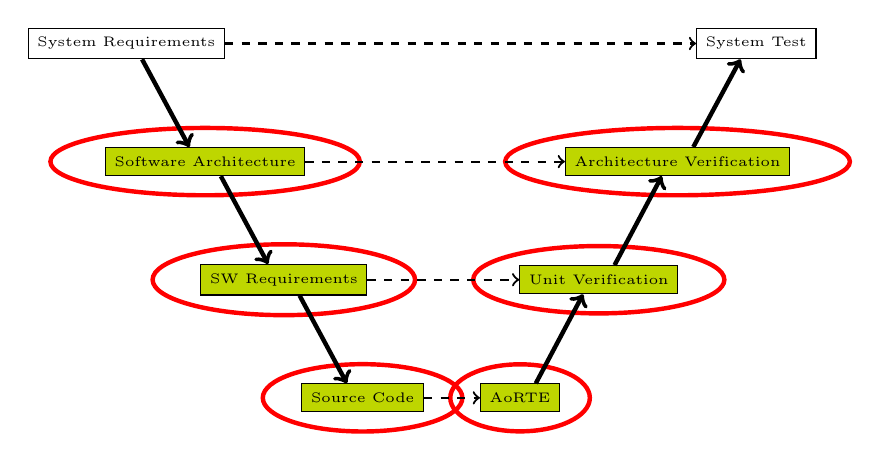
\begin{tikzpicture}[font=\tiny,y=0.95cm]

        % Create the Boundary Variable nodes
        \node[rectangle, draw] (sys_reqs) at (-4cm,-0cm) {System Requirements};
        \node<-2>[rectangle, draw] (code) at (-1cm,-4.5cm) {Source Code};
        \node<3->[rectangle, draw, fill, fill=AnSecondaryGreen] (code) at (-1cm,-4.5cm) {Source Code};
        \node<-3>[rectangle, draw] (aorte) at (1cm,-4.5cm) {AoRTE};
        \node<4->[rectangle, draw, fill, fill=AnSecondaryGreen] (aorte) at (1cm,-4.5cm) {AoRTE};
        \node<-4>[rectangle, draw] (sw_reqs) at (-2cm,-3cm) {SW Requirements};
        \node<5->[rectangle, draw, fill, fill=AnSecondaryGreen] (sw_reqs) at (-2cm,-3cm) {SW Requirements};
        \node<-5>[rectangle, draw] (unit_ver) at (2cm,-3cm) {Unit Verification};
        \node<6->[rectangle, draw, fill, fill=AnSecondaryGreen] (unit_ver) at (2cm,-3cm) {Unit Verification};
        \node<-6>[rectangle, draw] (arch) at (-3cm,-1.5cm) {Software Architecture};
        \node<7->[rectangle, draw, fill, fill=AnSecondaryGreen] (arch) at (-3cm,-1.5cm) {Software Architecture};
        \node<-7>[rectangle, draw] (arch_ver) at (3cm,-1.5cm) {Architecture Verification};
        \node<8->[rectangle, draw, fill, fill=AnSecondaryGreen] (arch_ver) at (3cm,-1.5cm) {Architecture Verification};
        \node[rectangle, draw] (sys_test) at (4cm,-0cm) {System Test};


        % Draw the system boundary using containers (more maintainable than using draw)
        \node<2>[ellipse, draw, red, ultra thick,fit=(code)] (circle_code) {};
        \node<3>[ellipse, draw, red, ultra thick,fit=(aorte)] (circle_aorte) {};
        \node<4,8>[ellipse, draw, red, ultra thick,fit=(sw_reqs)] (circle_sw_reqs) {};
        \node<5>[ellipse, draw, red, ultra thick,fit=(unit_ver)] (circle_unit_ver) {};
        \node<6>[ellipse, draw, red, ultra thick,fit=(arch)] (circle_arc) {};
        \node<7>[ellipse, draw, red, ultra thick,fit=(arch_ver)] (circle_arch_ver) {};

        % Draw the downward arrows
        \draw[ultra thick][->] ([xshift=0.2 cm]sys_reqs.south) to ([xshift=-0.2cm]arch.north) ;
        \draw[ultra thick][->] ([xshift=0.2 cm]arch.south) to ([xshift=-0.2cm]sw_reqs.north) ;
        \draw[ultra thick][->] ([xshift=0.2 cm]sw_reqs.south) to ([xshift=-0.2cm]code.north) ;

        % Draw the dashed arrows
        \draw[dashed, thick][->] (sys_reqs.east) to (sys_test.west) ;
        \draw[dashed, thick][->] (arch.east) to (arch_ver.west) ;
        \draw[dashed, thick][->] (sw_reqs.east) to (unit_ver.west) ;
        \draw[dashed, thick][->] (code.east) to (aorte.west) ;

        % Draw the upward arrows
        \draw[ultra thick][<-] ([xshift=-0.2 cm]sys_test.south) to ([xshift=0.2cm]arch_ver.north) ;
        \draw[ultra thick][<-] ([xshift=-0.2 cm]arch_ver.south) to ([xshift=0.2cm]unit_ver.north) ;
        \draw[ultra thick][<-] ([xshift=-0.2 cm]unit_ver.south) to ([xshift=0.2cm]aorte.north) ;
       

      \end{tikzpicture}
    \end{center}
  \end{changemargin}
\end{frame}

\section{What?}

\begin{frame}[fragile]{A very short introduction to formal verification}
   \begin{itemize}
      \item Source code is modelled formally
      \begin{itemize}
         \item Code converted to sets of verification conditions
         \item VCs contain hypotheses representing what is known
         \item and conclusions representing what must be demonstrated
      \end{itemize}
      \item Conclusions include: 
      \begin{itemize}
         \item Checks that run-time errors won't be raised
         \item Checks that contracts are met
      \end{itemize}
      \item Automatic theorem provers typically discharge \textgreater 95\% of VCs
   \end{itemize}
\end{frame}

\begin{frame}[fragile]{Verification Spectrum}
  \note[item]<1>{The following slides will walk through the verification spectrum with code examples.}
  \note[item]<1>{On the first slide, just explain that SPARK supports incremental analysis, ie you can apply each of the techniques incrementally.}
  \note[item]<1>{Reason for not having access types is because it complicates the analysis of aliasing}
  \note[item]<1>{Point out that 95\% of AoRTE VCs are discharged automatically by SPARK Pro 11 toolset}

  \lstdefinestyle{magic}{
    basicstyle=\tiny\tt,
    keywordstyle=\color{AnColour02},
    moredelim=**[is][{\btHL[fill=AnSecondaryYellow!50,name=error]}]{`}{`},
  }

  \begin{columns}
    \begin{column}{2cm}
      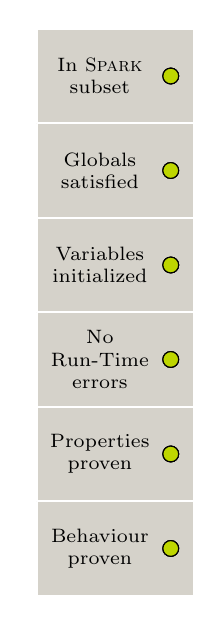
\begin{tikzpicture}[x=1cm,y=1.2cm]
        \tikzstyle{legend}=[font=\scriptsize,text badly centered,text width=1.6cm]
        \tikzstyle{unused}=[fill=white]
        \tikzstyle{error}=[fill=AnSecondaryRed]
        \tikzstyle{ok}=[fill=AnSecondaryGreen]

        \foreach \y in {1, 2, 3, 4, 5, 6} {
          \draw[fill=AnGrey01] (0, \y) -- (2, \y) -- (2, \y + 1) -- (0, \y + 1) -- (0, \y);
          \draw[white,thick]   (0, \y) -- (2, \y) -- (2, \y + 1) -- (0, \y + 1) -- (0, \y);
        }

        \node[legend] at (0.8, 6.5) {In \spark\ subset};
        \node[legend] at (0.8, 5.5) {Globals satisfied};
        \node[legend] at (0.8, 4.5) {Variables initialized};
        \node[legend] at (0.8, 3.5) {No Run-Time errors};
        \node[legend] at (0.8, 2.5) {Properties proven};
        \node[legend] at (0.8, 1.5) {Behaviour\\proven};

         % In SPARK subset
        \draw<1>[unused] (1.7, 6.5) circle (0.1cm);
        \draw<2>[error]   (1.7, 6.5) circle (0.1cm);
        \draw<3->[ok]     (1.7, 6.5) circle (0.1cm);

         % Globals satisfied
        \draw<-3>[unused]  (1.7, 5.5) circle (0.1cm);
        \draw<4>[error]    (1.7, 5.5) circle (0.1cm);
        \draw<5->[ok]      (1.7, 5.5) circle (0.1cm);

         % Variables initialized
        \draw<-5>[unused] (1.7, 4.5) circle (0.1cm);
        \draw<6>[error]   (1.7, 4.5) circle (0.1cm);
        \draw<7->[ok]     (1.7, 4.5) circle (0.1cm);

         % No RT errors
        \draw<-7>[unused] (1.7, 3.5) circle (0.1cm);
        \draw<8>[error]   (1.7, 3.5) circle (0.1cm);
        \draw<9->[ok]     (1.7, 3.5) circle (0.1cm);

         % Partially proven
        \draw<-9>[unused] (1.7, 2.5) circle (0.1cm);
        \draw<10>[error]   (1.7, 2.5) circle (0.1cm);
        \draw<11->[ok]     (1.7, 2.5) circle (0.1cm);

         % Fully proven
        \draw<-11>[unused] (1.7, 1.5) circle (0.1cm);
        \draw<12>[error]   (1.7, 1.5) circle (0.1cm);
        \draw<13->[ok]     (1.7, 1.5) circle (0.1cm);
      \end{tikzpicture}
    \end{column}

    \begin{column}{9cm}
      %\hrule

      \begin{onlyenv}<2>
      \begin{pxcode}[language=SPARK,style=magic,gobble=8]
        package Conference_Attendance
        is
           Max_Attendance : constant := 1000;
           type Count_T is range 0 .. Max_Attendance;
           type Counter_Access is access Count_T;

           procedure Inc_Counter (Counter : `Counter_Access`);

        end Conference_Attendance;

        package body Conference_Attendance
        is
           procedure Inc_Counter (Counter : `Counter_Access`)
           is
           begin
              Counter.all := Counter.all + 1;
           end Inc_Counter;

        end Conference_Attendance;

      \end{pxcode}
      \end{onlyenv}

      \begin{onlyenv}<3>
      \begin{pxcode}[language=SPARK,style=magic,gobble=8]
        package Conference_Attendance
        is
           Audience_Count, P_Count : Integer;

           procedure Inc_Audience (N : Integer)

        end Conference_Attendance;

        package body Conference_Attendance
        is
           procedure Inc_Audience (N : Integer)
           is
           begin
              Audience_Count := Audience_Count + N;
           end Inc_Audience;
        end Conference_Attendance;
      \end{pxcode}
      \end{onlyenv}


      \begin{onlyenv}<4>
      \begin{pxcode}[language=SPARK,style=magic,gobble=8]
        package Conference_Attendance
        is
           Audience_Count, P_Count : Integer;

           procedure Inc_Audience (N : Integer)
           with Global => (`In_Out => Audience_Count`);

        end Conference_Attendance;

        package body Conference_Attendance
        is
           procedure Inc_Audience (N : Integer)
           is
           begin
              `Audience_Count := N`;
           end Inc_Audience;
        end Conference_Attendance;
      \end{pxcode}
      \end{onlyenv}

      \begin{onlyenv}<5>
      \begin{pxcode}[language=SPARK,style=magic,gobble=8]
        package Conference_Attendance
        is
           Audience_Count, P_Count : Integer;

           procedure Inc_Audience (N : Integer)
           with Global => (`In_Out => Audience_Count`);

        end Conference_Attendance;

        package body Conference_Attendance
        is
           procedure Inc_Audience (N : Integer)
           is
           begin
              `Audience_Count := Audience_Count + N`;
           end Inc_Audience;
        end Conference_Attendance;
      \end{pxcode}
      \end{onlyenv}


      \begin{onlyenv}<6>
      \begin{pxcode}[language=SPARK,style=magic,gobble=8]
        package Conference_Attendance
        is
           Audience_Count, P_Count : Integer;

           procedure Inc_Audience (N : Integer)
           with Global => (In_Out => Audience_Count);

        end Conference_Attendance;

        package body Conference_Attendance
        is
           procedure Inc_Audience (N : Integer)
           is
           begin
              Audience_Count := `Audience_Count` + N;
           end Inc_Audience;
        end Conference_Attendance;
      \end{pxcode}
      \end{onlyenv}

      \begin{onlyenv}<7>
      \begin{pxcode}[language=SPARK,style=magic,gobble=8]
        package Conference_Attendance
        is
           Audience_Count, P_Count : Integer := `0`;

           procedure Inc_Audience (N : Integer)
           with Global => (In_Out => Audience_Count);

        end Conference_Attendance;

        package body Conference_Attendance
        is
           procedure Inc_Audience (N : Integer)
           is
           begin
              Audience_Count := Audience_Count + N;
           end Inc_Audience;
        end Conference_Attendance;
      \end{pxcode}
      \end{onlyenv}

      \begin{onlyenv}<8>
      \begin{pxcode}[language=SPARK,style=magic,gobble=8]
        package Conference_Attendance
        is
           Audience_Count, P_Count : Integer := 0;

           procedure Inc_Audience (N : Integer)
           with Global => (In_Out => Audience_Count);

        end Conference_Attendance;

        package body Conference_Attendance
        is
           procedure Inc_Audience (N : Integer)
           is
           begin
              Audience_Count := `Audience_Count + N`;
           end Inc_Audience;
        end Conference_Attendance;
      \end{pxcode}
      \end{onlyenv}

      \begin{onlyenv}<9>
      \begin{pxcode}[language=SPARK,style=magic,gobble=8]
        package Conference_Attendance
        is
           `Max_Attendance : constant := 1000;`
           `type Count_T is range 0 .. Max_Attendance;`

           Audience_Count, Presenter_Count : Count_T := 0;

           procedure Inc_Audience (N : Integer)
           with Global => (In_Out => Audience_Count),
                `Pre    => (0 <= N, Audience_Count + N <= Max_Attendance);`

        end Conference_Attendance;

        package body Conference_Attendance
        is
           procedure Inc_Audience (N : Integer)
           is
           begin
              Audience_Count := Audience_Count + N;
           end Inc_Audience;
        end Conference_Attendance;
      \end{pxcode}
      \end{onlyenv}

      \begin{onlyenv}<10>
      \begin{pxcode}[language=SPARK,style=magic,gobble=8]
        package Conference_Attendance
        is
           Max_Attendance : constant := 1000;
           type Count_T is range 0 .. Max_Attendance;

           Audience_Count, Presenter_Count : Count_T := 0;

           procedure Inc_Audience (N : Integer)
           with Global => (In_Out => Audience_Count),
                Pre    => 0 <= N and Audience_Count + N <= Max_Attendance,
                `Post   => Audience_Count > Audience_Count'Old;`

        end Conference_Attendance;

        package body Conference_Attendance
        is
           procedure Inc_Audience (N : Integer)
           is
           begin
              Audience_Count := Audience_Count `-` N;
           end Inc_Audience;
        end Conference_Attendance;
      \end{pxcode}
      \end{onlyenv}

      \begin{onlyenv}<11>
      \begin{pxcode}[language=SPARK,style=magic,gobble=8]
        package Conference_Attendance
        is
           Max_Attendance : constant := 1000;
           type Count_T is range 0 .. Max_Attendance;

           Audience_Count, Presenter_Count : Count_T := 0;

           procedure Inc_Audience (N : Integer)
           with Global => (In_Out => Audience_Count),
                Pre    => 0 <= N and Audience_Count + N <= Max_Attendance,
                Post   => Audience_Count > Audience_Count'Old;

        end Conference_Attendance;

        package body Conference_Attendance
        is
           procedure Inc_Audience (N : Integer)
           is
           begin
              Audience_Count := Audience_Count `+` N;
           end Inc_Audience;
        end Conference_Attendance;
      \end{pxcode}
      \end{onlyenv}


      \begin{onlyenv}<12>
      \begin{pxcode}[language=SPARK,style=magic,gobble=8]
        package Conference_Attendance
        is
           Max_Attendance : constant := 1000;
           type Count_T is range 0 .. Max_Attendance;
           Audience_Count, Presenter_Count : Count_T := 0;
           Presenter_Set : Name_Sets.Set;

           procedure Inc_Audience (N : Integer)
           with Global => (In_Out => Audience_Count),
                Pre    => 0 <= N and Audience_Count + N <= Max_Attendance,
                Post   => `Audience_Count = Audience_Count'Old + N`;

        end Conference_Attendance;

        package body Conference_Attendance
        is
           procedure Inc_Audience (N : Integer)
           is
           begin
              Audience_Count := `Audience_Count - N`;
           end Inc_Audience;

        end Conference_Attendance;
      \end{pxcode}
      \end{onlyenv}

      \begin{onlyenv}<13>
      \begin{pxcode}[language=SPARK,style=magic,gobble=8]
        package Conference_Attendance
        is
           Max_Attendance : constant := 1000;
           type Count_T is range 0 .. Max_Attendance;
           Audience_Count, Presenter_Count : Count_T := 0;
           Presenter_Set : Name_Sets.Set;

           procedure Inc_Audience (N : Integer)
           with Global => (In_Out => Audience_Count),
                Pre    => 0 <= N and Audience_Count + N <= Max_Attendance,
                Post   => `Audience_Count = Audience_Count'Old + N`;

        end Conference_Attendance;

        package body Conference_Attendance
        is
           procedure Inc_Audience (N : Integer)
           is
           begin
              Audience_Count := Audience_Count `+` N;
           end Inc_Audience;

        end Conference_Attendance;
      \end{pxcode}
      \end{onlyenv}

      \begin{onlyenv}<14>
      \begin{pxcode}[language=SPARK,style=magic,gobble=8]
        package Conference_Attendance
        is
           Max_Attendance : constant := 1000;
           type Count_T is range 0 .. Max_Attendance;
           Audience_Count, Presenter_Count : Count_T := 0;
           Presenter_Set : Name_Sets.Set;

           procedure Inc_Audience (N : Integer)
           with Global => (In_Out => Audience_Count),
                Pre    => 0 <= N and Audience_Count + N <= Max_Attendance,
                Post   => Audience_Count = Audience_Count'Old + N;

        end Conference_Attendance;

        package body Conference_Attendance
        is
           procedure Inc_Audience (N : Integer)
           is
           begin
              Audience_Count := Audience_Count + N;
           end Inc_Audience;

        end Conference_Attendance;
      \end{pxcode}
      \end{onlyenv}




%           procedure Inc_Presenter(Name : String)
%           with Global => (In_Out => Presenter_Count, Presenter_List),
%                Pre    => (Presenter_Count < Max_Attendance);
%                Post   => (Presenters_Set.Insert(Name) and 
%                           Presenter_Count = Presenters_Set.Count);
%           ...



      %\hrule
    \end{column}
  \end{columns}

\end{frame}

\begin{frame}[fragile]{Combining proof and test overview}
  \note[item]<1>{Key message: neither full proof, nor full test is sufficient}
  \note[item]<1>{item talk about system test as out of scope}
  \note[item]<1>{Explain that we are considering full functional proof/test, not just RTE proof.}
  \begin{changemargin}{-0.75cm}{-0.75cm}
    \begin{center}
      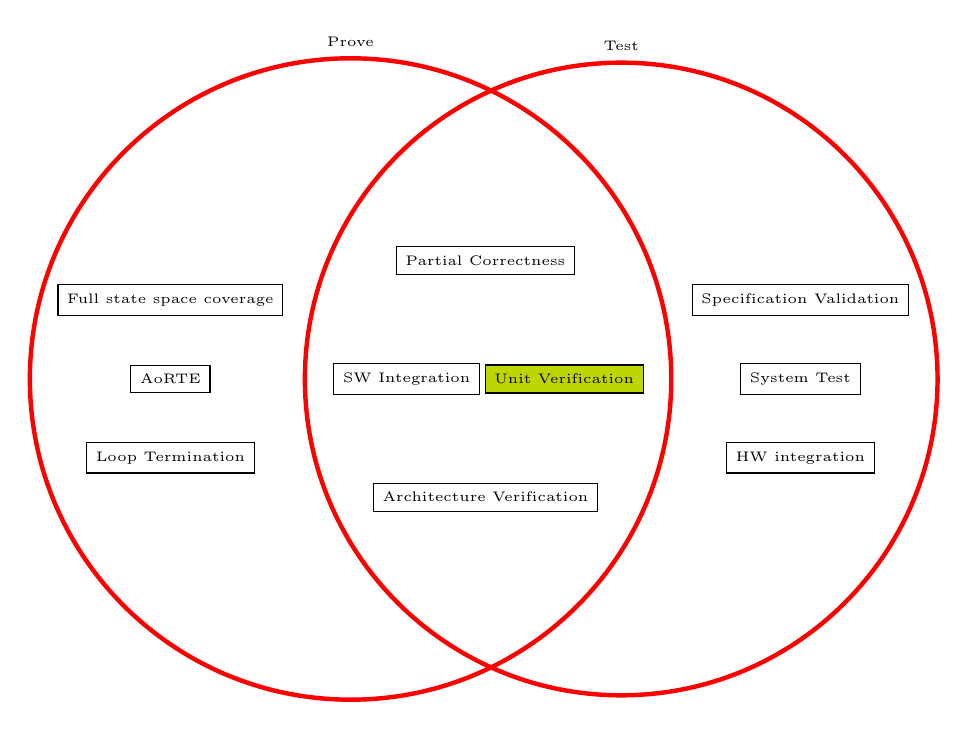
\begin{tikzpicture}[font=\tiny,y=0.95cm]

        % Create the test only nodes
        \node[rectangle, draw] (spec_val) at (4.0cm, -0.5cm) {Specification Validation};
        \node[rectangle, draw] (sys_test) at (4cm,-1.5cm) {System Test};
        \node[rectangle, draw] (hw_int) at (4.0cm,-2.5cm) {HW integration};

        % Create the proof only nodes
        \node[rectangle, draw] (state_coverage) at (-4.0cm,-0.5cm) {Full state space coverage};
        \node[rectangle, draw] (rte) at (-4cm,-1.5cm) {AoRTE};
        \node[rectangle, draw] (term) at (-4.0cm,-2.5cm) {Loop Termination};

        % Create the proof and test nodes
        \node[rectangle, draw] (part) at (-0cm, -0.0cm) {Partial Correctness};
        \node[rectangle, draw] (sw_int) at (-1cm,-1.5cm) {SW Integration};
        \node<-4>[rectangle, draw] (unit_ver) at (1cm,-1.5cm) {Unit Verification};
        \node<5->[rectangle, draw, fill, fill=AnSecondaryGreen] (unit_ver) at (1cm,-1.5cm) {Unit Verification};
        \node[rectangle, draw] (arch_ver) at (0cm,-3.0cm) {Architecture Verification};


        % Draw the system boundary using containers (more maintainable than using draw)
        \node<2,4->[circle, label=above:{Prove}, draw, red, ultra thick,inner sep=0pt,fit=(unit_ver) (state_coverage) (term)(rte) (arch_ver) (part)] (circle_proof) {};
        \node<3->[circle, label=above:{Test}, draw, red, ultra thick,inner sep=0pt, fit=(sw_int) (spec_val) (sys_test)(hw_int) (arch_ver) (part)] (circle_test) {};

      \end{tikzpicture}
    \end{center}
  \end{changemargin}
\end{frame}

\begin{frame}[fragile]{Proof and Test Scenario Summary}
\note[item]{We've looked at valid combinations of proof or test against the level of formal specification}
\note[item]{`Proof only' is only an option when the requirements are fully specified in contracts}
\begin{center}
\begin{tabular}{p{4.3cm} | c | c | c }
    & Fully & Partially & Can't \\
    & specify & specify & specify \\
  \hline
  Only prove & HR & NR & NR \\
  \hline
  Only test &  NR &  NR & M \\
  \hline
  \raggedright Prove some and test some & R & R & R \\
  \hline
  Test to debug contracts & - & - & - \\
\end{tabular}

\vspace{1cm}
M: Mandatory; HR: Highly Recommended; R: Recommended; 

''-'': Optional; NR: Not Recommended.

\end{center}

\end{frame}

\begin{frame}[fragile]{Only test}
  \note[item]<1>{Integer square root can be simple and proven but inefficient}
  \note[item]<1>{Bit-shift algorithms much more efficient but hard to prove}
  \begin{itemize}
     \item Contracts could be hard to formalize eg:
     \begin{itemize}
        \item Interface with hardware
        \item Timing properties
     \end{itemize}
     \item Implementation may rely on obtuse minimalist algorithms
  \end{itemize}
  \begin{pxcode}[language=SPARK,style=magic,gobble=0]

  --  Calculates the square root of X
  function Sqrt (X : in Natural) return Natural 
  with Post =>
         (Sqrt'Result * Sqrt'Result) <= X and
          (Sqrt'Result + 1) * (Sqrt'Result + 1) > X;



  \end{pxcode}
\end{frame}
\begin{frame}[fragile]{Example unit testing tool}
  \note{Using modern unit test tools makes it easier to put together harnesses but users still need to define the test inputs and expected outcomes. Also, unit testing will often not cover the entire state space.}
  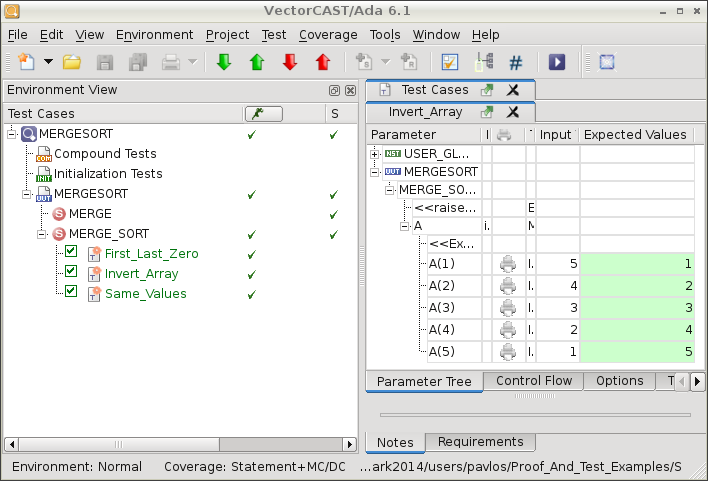
\includegraphics[width=\textwidth]{VectorCAST_resized.jpg}
\end{frame}

\begin{frame}[fragile]{Test to verify contracts}
  \note[item]{Key message: When provers aren't capable, execute contract over all cases}
  \note[item]{We plan to be able to automatically prove this specific type of contract}
  \note[item]{Nested quantifiers (for all, for some) are the problem}
  \begin{itemize}
     \item Some contracts are difficult to prove ...
  \end{itemize}

  \begin{pxcode}[language=SPARK,style=magic,gobble=3]

      -- Check that all states are reachable
      pragma Assert
        (for all Final_State in States_T =>
           (for some Initial_State in States_T =>
                (for some A_Trigger in Triggers_T =>
                     (Final_State = My_SM(Initial_State, A_Trigger)))));
  \end{pxcode}

  \begin{itemize}
     \item ... but easy to test.
  \end{itemize}

\end{frame}

\begin{frame}[fragile]{Test to debug contracts}
  \note{Key message: Executing contracts is a great way of checking them}
  \begin{itemize}
     \item Execute precondition to check it isn't too strong
     \item Execute assertions and postcondition to check they hold under normal conditions
     \item Use pragma assert like a "debug" statement for contracts
  \end{itemize}
\end{frame}

\begin{frame}[fragile]{Test to debug contracts - using assert to debug}
  \begin{pxcode}[language=SPARK,style=magic,gobble=3]
   procedure Progress_SM(Trigger : in Triggers_T)
     with Refined_Global => (in_out => State)
   is
   begin

      if Trigger = Btn_Pressed then
         if State = Start then
            Set_State(Progress);
         elsif State = Progress or State = Finish then
            Set_State(Finish);
         else
            Set_State(Invalid_State);
         end if;

         `pragma Assert (Get_State = My_SM(Old_State, Trigger));`

      elsif Trigger = Btn_Start then
         Set_State(Start);

      elsif Trigger = Btn_Finish then
         Set_State(Finish);

      elsif Trigger = Invalid_Trigger then
         Set_State(Invalid_State);

      end if;

   end Progress_SM;
  \end{pxcode}
  \note[item]{Assert statements can be used to check specific paths through the code.}
  \note[item]{The Show Path functionality would be better for this specific example.}
\end{frame}

\begin{frame}[fragile]{Only prove - specification}
  \note[item]{Key message: Proof isn't just possible, it is often easier than test!}
  \note[item]{This is an example generated for a client. The message is, we put this specification together and then wrote an implementation and the tools fully proved consistency without any strengthen of preconditions, addition of asserts and the VCs didn't even need to be inspected.}
  \note[item]{Say that the original code was C}
  \note[item]{Make it clear that this was in response to a program freezing during customer integration testing because some states had not been fully defined - it is key to highlight this as it will (I hope) be a good example of where SPARK can make a real difference}
  \begin{pxcode}[language=SPARK,style=magic,gobble=3]
   function My_SM(State : in States_T; Trigger: in Triggers_T)
                  return States_T is
     (case State is
         when Start =>
         (if    Trigger = Btn_Start    then Start
          elsif Trigger = Btn_Finish   then Finish
          elsif Trigger = Btn_Pressed  then Progress
          elsif Trigger = Btn_Released then Start
          else                              Invalid_State),
         when Progress =>
         (if    Trigger = Btn_Start    then Start
          elsif Trigger = Btn_Finish   then Finish
          elsif Trigger = Btn_Pressed  then Finish
          elsif Trigger = Btn_Released then Progress
          else                              Invalid_State),
         when Finish =>
         (if    Trigger = Btn_Start    then Start
          elsif Trigger = Btn_Finish   then Finish
          elsif Trigger = Btn_Pressed  then Finish
          elsif Trigger = Btn_Released then Finish
          else                              Invalid_State),
         when Invalid_State =>
         (if    Trigger = Btn_Start    then Start
          elsif Trigger = Btn_Finish   then Finish
          else                              Invalid_State));

  \end{pxcode}
\end{frame}

\begin{frame}[fragile]{Only prove - implementation}
  \begin{changemargin}{-0.75cm}{-0.75cm}
    \begin{center}
      \begin{tikzpicture}[font=\huge,y=0.95cm]
          \node<2>[draw, rectangle, fill=AnSecondaryGreen, rotate=25] at (0,0.0) {Proven};

          \node {%
              \begin{minipage}[t!]{0.5\textwidth}
  \begin{pxcode}[language=SPARK,style=magic,gobble=3]
   procedure Progress_SM(Trigger : in Triggers_T)
     with Refined_Global => (in_out => State)
   is
   begin

      if Trigger = Btn_Pressed then
         if State = Start then
            Set_State(Progress);
         elsif State = Progress or State = Finish then
            Set_State(Finish);
         else
            Set_State(Invalid_State);
         end if;

      elsif Trigger = Btn_Start then
         Set_State(Start);

      elsif Trigger = Btn_Finish then
         Set_State(Finish);

      elsif Trigger = Invalid_Trigger then
         Set_State(Invalid_State);

      end if;

   end Progress_SM;
  \end{pxcode}

    \end{minipage}
    };
      \end{tikzpicture}
    \end{center}
  \end{changemargin}
\end{frame}

% \begin{frame}[fragile]{Only prove - quick tips for improving provability}
%   \note{Describe when proof is easy/hard (linear/non-linear arithmetic) (logic vs computations?)}
%   \note[item]{should we remove the bullet about cyclomatic complexity?}
%   \begin{itemize}
%         \item Re-use expression functions in implementation
%         \item Reduce cyclomatic complexity
%         \item Strengthen pre-conditions
%         \item Add assertions to the code
%         \item Increase prover time out
%   \end{itemize}
% \end{frame}

\begin{frame}[fragile]{Prove and test: \newline Parallelise verification using contracts}
  \begin{changemargin}{-0.75cm}{-0.75cm}
    \begin{center}
      \begin{tikzpicture}[font=\huge,y=0.95cm]

%        \node (main) at (-3cm, 0cm) {%
%         \begin{minipage}[t!]{0.25\textwidth}
%
%          \begin{pxcode}[language=SPARK,style=magic,gobble=12]
%            procedure Main
%            is
%            begin
% 
%               Inc_Audience(3);
%               Inc_Audience(2);
%               Inc_Audience(1);
%
%            end Progress_SM;
%           \end{pxcode}
%          \end{minipage} } ;

        \node (sort) at (-0cm, -1.5cm) {%
         \begin{minipage}[t!]{0.5\textwidth}
          \begin{onlyenv}<1>
            \begin{pxcode}[language=SPARK,style=magic,gobble=15]
               function Has_Duplicates(Table : in Array_Type)
                  return Boolean;
             \end{pxcode}
          \end{onlyenv}

          \begin{onlyenv}<2->
           \begin{pxcode}[language=SPARK,style=magic,gobble=15]
               function Has_Duplicates(Table : in Array_Type)
                  return Boolean
               with Post => 
                      for all i in Array_Type'Range => 
                         for all j in Array_Type'Range => 
                            if i /= j then Table(i) /= Table(j);

           \end{pxcode}
          \end{onlyenv}
         \end{minipage} };


        \node (perm) at (-4cm, -5.5cm) {%
         \begin{minipage}[t!]{0.25\textwidth}
          \begin{onlyenv}<-2>
            \begin{pxcode}[language=SPARK,style=magic,gobble=15]
               procedure Sort(A : in out Array_Type);
             \end{pxcode}
          \end{onlyenv}

          \begin{onlyenv}<3->
           \begin{pxcode}[language=SPARK,style=magic,gobble=15]
               procedure Sort(A : in out Array_Type) 
               with Post => 
                       (for all I in 
                          Array_Type'First .. 
                             Array_Type'Last - 1 =>
                             A(I) <= A (I + 1));
           \end{pxcode}
          \end{onlyenv}
         \end{minipage} };

        \node (ordered) at ( 3cm, -5.5cm) {%
         \begin{minipage}[t!]{5cm}
          \begin{onlyenv}<-2>
           \begin{pxcode}[language=SPARK,style=magic,gobble=13]
             function Ordered_Has_Duplicates(A : Array_T)
                return Boolean;
           \end{pxcode}
          \end{onlyenv}

          \begin{onlyenv}<3>
           \begin{pxcode}[language=SPARK,style=magic,gobble=13]
             function Ordered_Has_Duplicates(A : Array_T)
                  return Boolean
               with Post => 
                       (for all I in 
                          Array_Type'First .. 
                             Array_Type'Last - 1 =>
                             A(I) /= A(I + 1));

           \end{pxcode}
          \end{onlyenv}
         \end{minipage} };



        \draw[ultra thick][->] (sort.south) to ([xshift= 0.5cm]perm.north) ;
        \draw[ultra thick][->] (sort.south) to ([xshift=-0.5cm]ordered.north) ;

      \end{tikzpicture}
    \end{center}
  \end{changemargin}
\end{frame}


%           procedure Inc_Audience (N : Count_T)
%           with Global => (In_Out => Audience_Count),
%                Pre    => (0 <= N),
%                Post   => (Audience_Count = 
%                              Max(Audience_Count'Old + N, Count_T'Last));




\begin{frame}[fragile]{Prove and test}
  \note{Key message: Mixing of proof and test most effective method}
  \begin{itemize}
     \item Lowest-level operations often prove automatically
     \item Always start by attempting to prove rather than test
     \item If you can't fully prove behaviour use "Assume"
     \begin{itemize}
        \item Assume statements are checked at run-time
     \end{itemize}
     \item Always prove properties that are hard to fully test eg
     \begin{itemize}
        \item Run-Time Errors 
        \item Safety properties
     \end{itemize}
     
  \end{itemize}
\end{frame}



\begin{frame}[fragile]{Conclusions}
  SPARK 2014 supports predictable software development by:
  \begin{itemize}
     \item \emph{improving quality} of legacy code through incremental analysis
     \item \emph{reducing effort} by replacing unit test with automated proof
     \item \emph{reducing time} by parallelising unit verification
  \end{itemize}

  \vspace{0.3cm}

  What next?
  \begin{itemize}
     \item Try testing your code using Ada 2012 contracts
     \item Visit www.spark-2014.org
     \item SPARK 2014 Beta tools are available - ask us for more info
     \item Ask questions now, come and chat or send me an e-mail: andrew.hawthorn@altran.com
  \end{itemize}

  \vspace{0.3cm}

  \begin{center}
     
\includegraphics[width=5cm]{partnership_logo_big.png}
  \end{center}
\end{frame}


\end{document}

